\documentclass[11pt,titlepage]{article}
\usepackage{Preamble}

\begin{document}

\begin{titlepage}
    \newgeometry{margin=3cm}
	\centering
    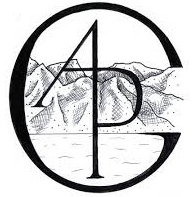
\includegraphics[width=0.3\linewidth]{gap.png}\\[0.25cm] 	% University Logo
    \textsc{\LARGE Gymnase Auguste Piccard}\\ \vspace{\fill}
    \textbf{\textsc{\fontsize{40}{40}\selectfont Champ magnétique émis par un solénoïde}}\\ \vspace{\fill}		
	\textsc{\LARGE Option spécifique physique, 3M8}\\[0.4cm]
	\rule{\linewidth}{0.2 mm} \\[0.5 cm]
	Julien Bricka, Romain Blondel \\[2cm] \today
\end{titlepage}
\restoregeometry%

\thispagestyle{numberonly}
\begin{summary}
\section*{But}
% Résumer en quelques lignes le but du TP
% Évoquer les méthodes utilisée

Le but de ce travail est de mesurer puis comparer des modèles du champ magnétique créé par le courant parcourant un solénoïde.

\end{summary}

\section{Introduction}
\subfile{1-Introduction}

\section{Principe de mesure et description}
\subfile{2-Methods}

\section{Résultats et calculs}
\subfile{3-Results}

\section{Discussion des résultats}
\subfile{4-Discussion}

\section{Conclusion}
\subfile{5-Conclusion}

\end{document}
